\label{chap:formative-study}

Following the literature-based motivation for a hybrid graph-table interface, this thesis conducted a formative, user-centred study to ground the design in students' real planning practices and to derive implementable requirements. The study used an interactive but non-functional prototype as an elicitation artefact to make workflows, expectations, and missing functionality tangible to participants. It operates at levels~1 and~2 of Munzner's \gterm{nested-model}{nested model}: domain problem characterisation, which it shares with the review of Chapter~\ref{chap:related-work}, and data and task abstraction, which the specification of Section~\ref{chap:from-themes-to-requirements} produces (Chapter~\ref{chap:methodology}, Section~\ref{sec:paradigm}).

This chapter answers the first research question:

\begin{quote}
\textit{What are students' needs and resulting requirements for a hybrid graph-table interface that supports programme-level study planning and understanding of curriculum structure and course dependencies?}
\end{quote}

The outcome of this chapter is a ranked set of themes, each standing for a recurring planning-related need, and, derived from them in Section~\ref{chap:from-themes-to-requirements}, the features-and-requirements specification that design and development build on (Chapters~\ref{chap:design} and~\ref{chap:implementation}) and the evaluation reports against (Chapter~\ref{chap:evaluation}).

% ------------------------------------------------------------
\section{Study Goal and Guiding Questions}
\label{sec:study-goal}

The goal of the formative study was to understand how students currently plan their study programme at a programme level, identify pain points and breakdowns in current tools and practices, and gather input on features students would want when confronted with the concept of a hybrid graph-table interface.

\subsection{Guiding Questions}

To operationalise this goal, the interviews were guided by the following questions:

\begin{itemize}
    \item \textbf{Current practice:} How do students currently plan upcoming semesters and their overall programme progress, and which resources or tools do they use?
    \item \textbf{Decision pain points:} Which parts of study planning are effortful, error-prone, or frustrating?
    \item \textbf{Information needs:} What information do students need at decision points?
    \item \textbf{Concept fit of a hybrid interface:} Where would a graph view help (structure, dependencies, exploration), and where would a table help (semester allocation, workload overview)?
    \item \textbf{Requirement implications:} Which concrete capabilities should the tool provide to reduce planning effort and increase confidence, and what should explicitly remain out of scope?
\end{itemize}

% ------------------------------------------------------------
\section{Prototype as Elicitation Artefact}
\label{sec:prototype-elicitation}

\paragraph{Purpose of the prototype in the study.}
The prototype gave participants something concrete to react to, instead of asking them to imagine an abstract planning tool. Rather than discussing study planning only at an abstract level, participants could react to visible interface elements, anticipated workflows, and concrete interaction concepts. It was not intended to evaluate visual polish, implementation quality, or system performance.
The prototype's underlying concept, a hybrid interface combining a node-link graph with a semester table, was not itself derived from these interviews. As stated in the Methodology chapter (Section~\ref{sec:overall-assumptions}), the need for this combination is motivated by the related-work review (Chapter~\ref{chap:related-work}) and treated as a starting assumption going into the formative study, not as a hypothesis tested against alternatives. The formative study's role was accordingly to elicit requirements \emph{within} this hybrid concept, including which panels, encodings, and interactions it should have.

\paragraph{What the prototype represented.}
The prototype represented the hybrid concept as three linked interaction spaces. The \emph{\gterm{table-view}{Table View}} (Figure~\ref{fig:prototype-tableview}) laid the plan out as semester lanes fed from a searchable catalogue sidebar, with running totals of European Credit Transfer and Accumulation System (\gterm{ects}{ECTS}) credits per semester. The \emph{\gterm{graph-view}{Graph View}} (Figure~\ref{fig:prototype-graphview}) showed the same curriculum as a node-link structure of \gterm{exam-subject}{exam subjects}, modules and courses, with filters for what to display. Recommendation actions (Figure~\ref{fig:prototype-recommendation}) were reachable from both views, so that a suggested course could be inspected and placed without leaving the surface the participant was already on. What mattered for elicitation is that both views operate on one plan, and that moving between them is possible at any point; the visual particulars are secondary and are left to the figures.

\begin{figure}[htbp]
    \centering
    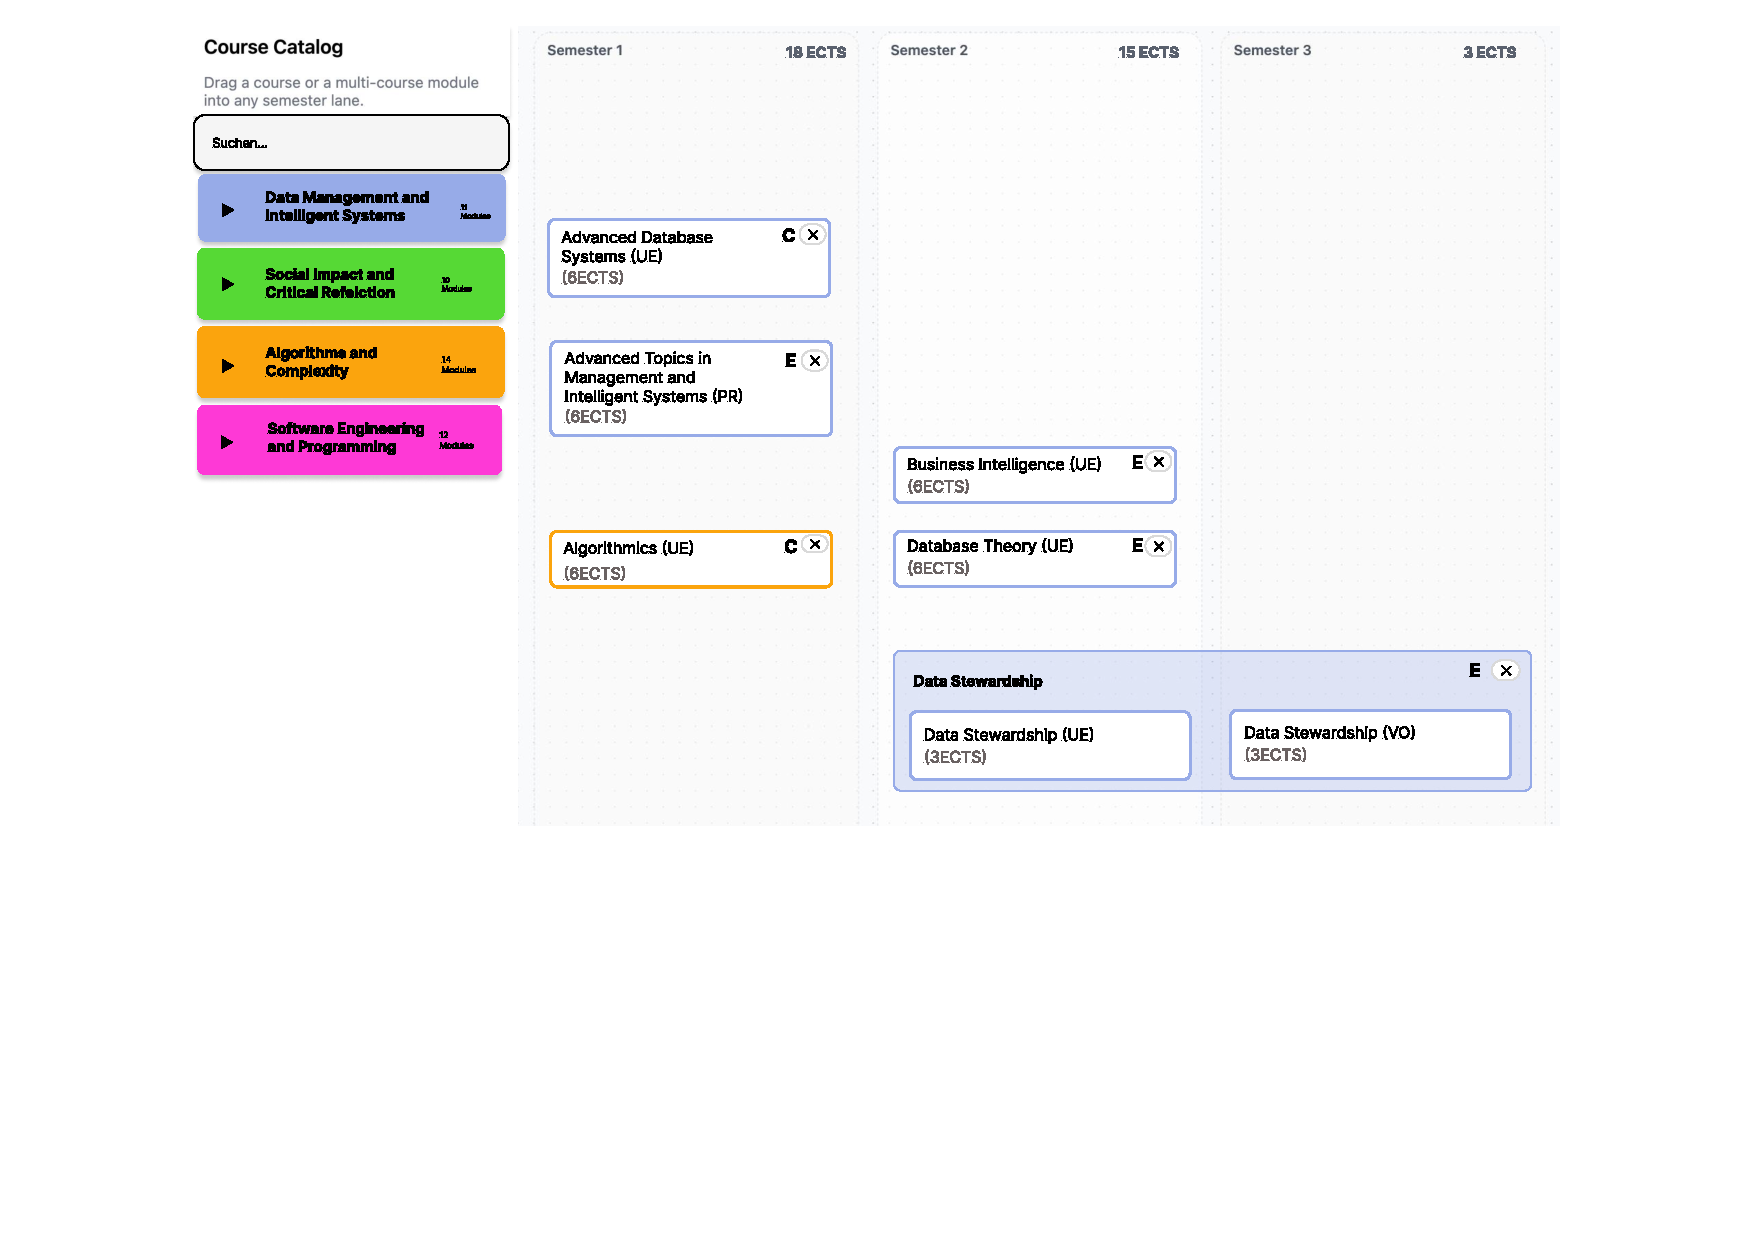
\includegraphics[width=\textwidth]{pictures/Prototype_TableView.pdf}
    \caption{Table View of the prototype: semester columns with running ECTS totals, a searchable catalogue sidebar, and courses and grouped modules placed as movable cards.}
    \label{fig:prototype-tableview}
\end{figure}

\begin{figure}[htbp]
    \centering
    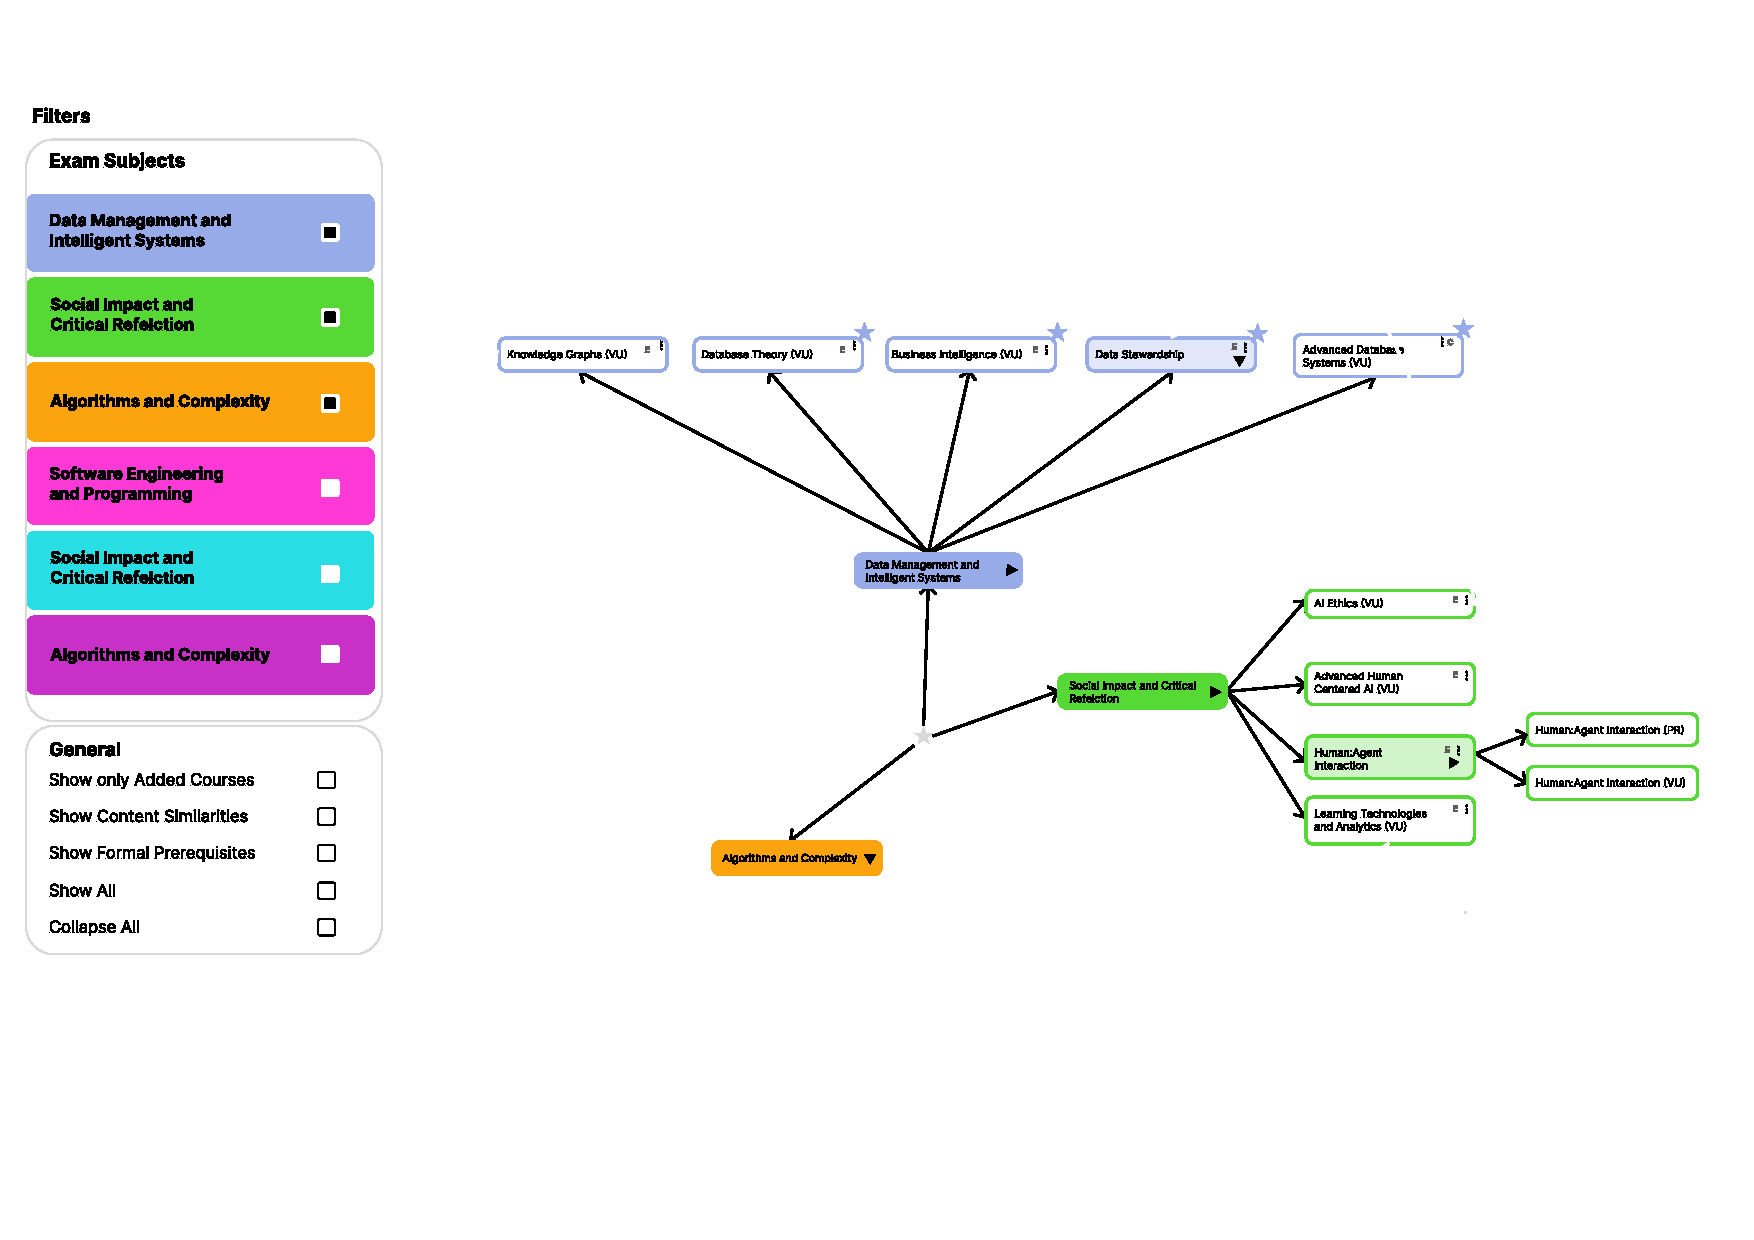
\includegraphics[width=\textwidth]{pictures/Prototype_GraphView.pdf}
    \caption{Graph View of the prototype: exam subjects, modules, and courses as colour-coded nodes, with filter controls, planned-course markers, and collapsible branches.}
    \label{fig:prototype-graphview}
\end{figure}

\begin{figure}[htbp]
    \centering
    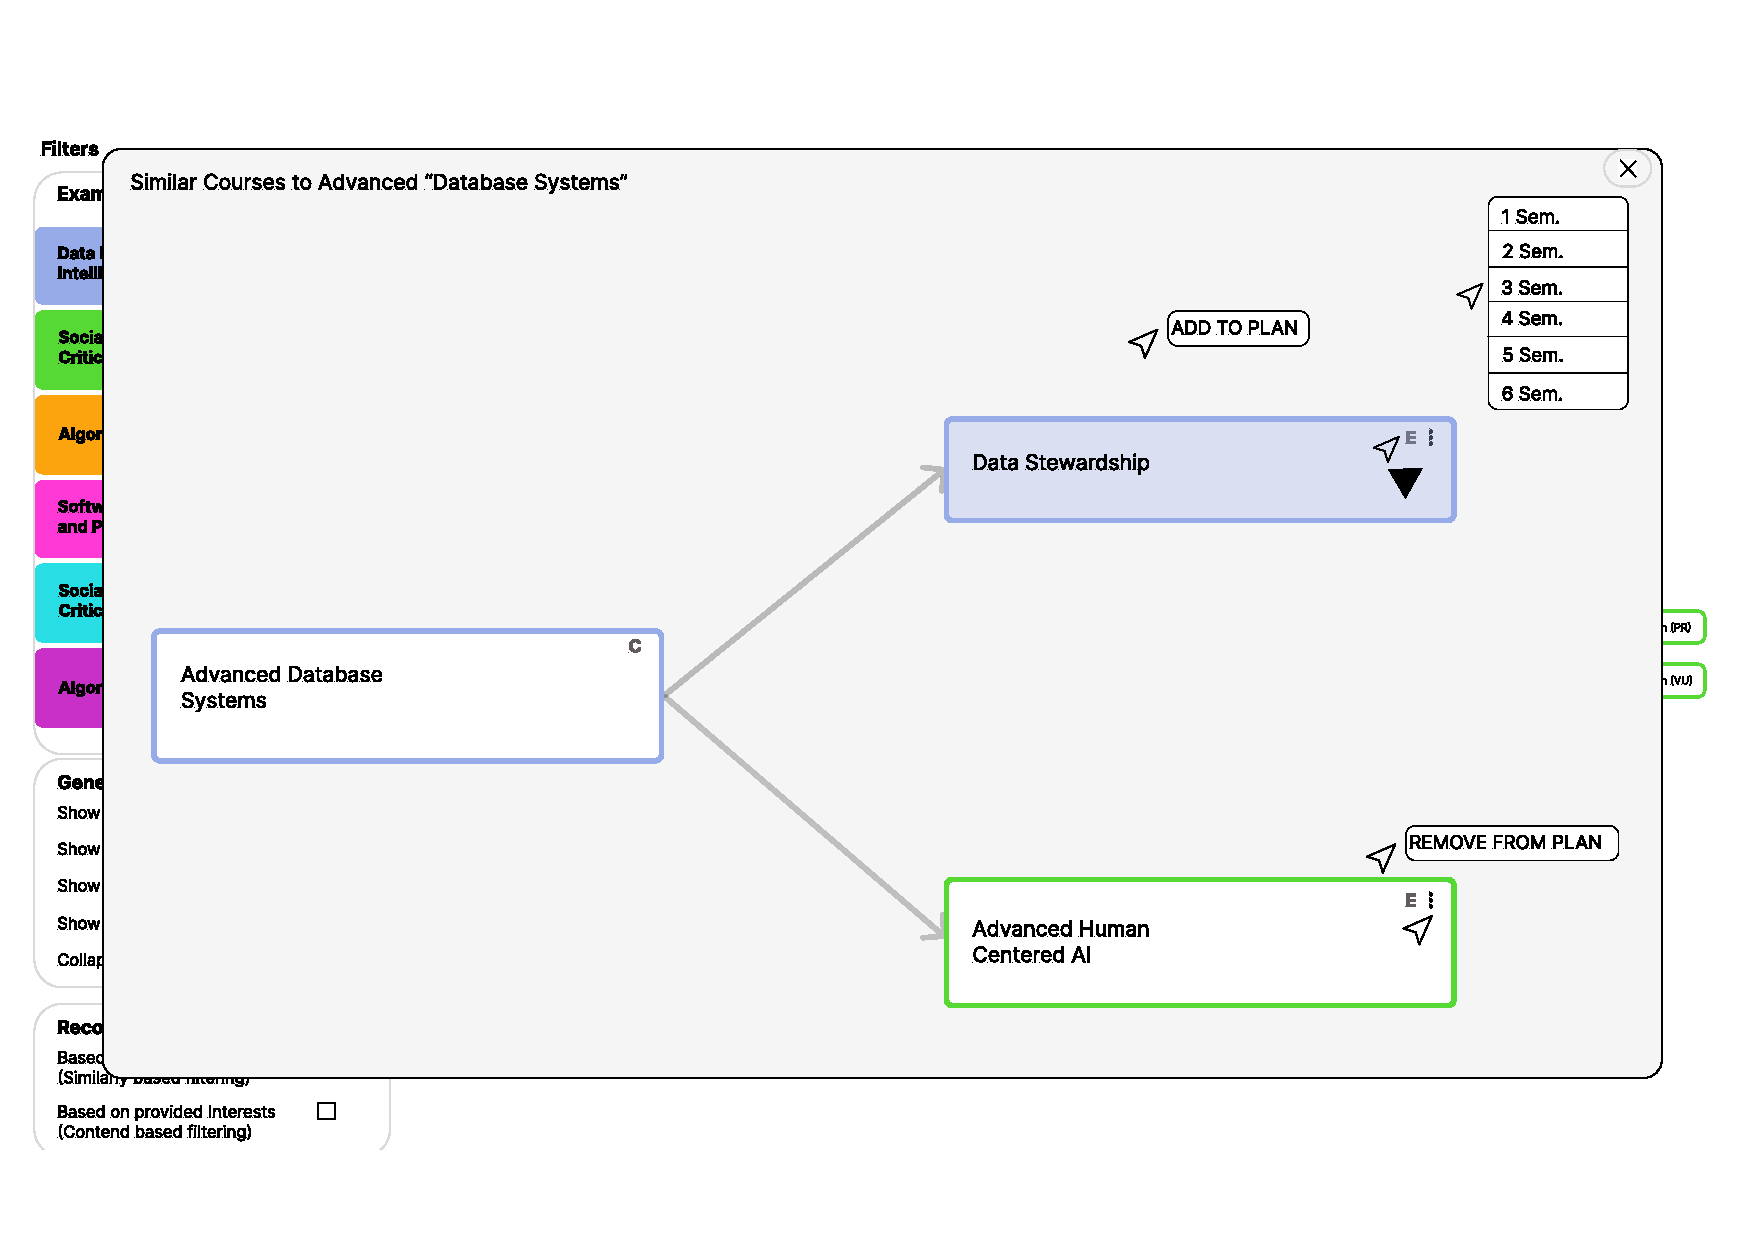
\includegraphics[width=\textwidth]{pictures/Prototype_SimilarCourses.pdf}
    \caption{Recommendation concept in the prototype: a focal course shown with related courses, add and remove actions, and a semester-selection control bridging into the plan.}
    \label{fig:prototype-recommendation}
\end{figure}

\paragraph{What the prototype did not represent.}
The prototype was visually detailed but not a functional system: it had no backend, no persistent data model, and no live rule-checking. Controls such as \enquote{Show Formal Prerequisites} and the recommendation actions were conceptual prompts for discussion, not validated computational features, and the recommendation views tested participants' expectations and acceptance conditions, not the quality of an actual algorithm. It also covered only a bounded subset of programmes and curriculum structures, so feedback about missing coverage was treated as a scope limitation of the elicitation artefact rather than a flaw in the interaction concept. In sum, the prototype functioned as a requirements-elicitation device for design and workflow discussion, not as a summative usability or system-performance evaluation instrument.

% ------------------------------------------------------------
\section{Participants and Recruitment}
\label{sec:participants-recruitment}

The formative study included six students from the Faculty of Informatics at TU~Wien: three Bachelor's students (Computer Science) and three Master's students (Software Engineering). The split was chosen to obtain perspectives at different degrees of curriculum familiarity and under different planning constraints, since a Bachelor's student working through broad foundational requirements and a Master's student choosing among specialised electives face different problems. Participants were eligible if they were enrolled in one of these two programmes, which is the population the tool is intended for.

With six participants from a single faculty, the aim was breadth of needs discovery rather than representativeness. The specification derived in Section~\ref{chap:from-themes-to-requirements} should accordingly be read as what this population needed, not as a statistically generalisable account of student planning.

\section{Procedure}
\label{sec:procedure}

Each session was a semi-structured interview combined with a think-aloud walkthrough of the prototype, run to a fixed plan of four phases: welcome and consent, current planning behaviour, prototype exploration, and reflection and wrap-up. Participants were asked for consent to audio recording before any questions, were told that the prototype was non-functional and that its gaps were the point of discussion, and were prompted to think aloud throughout the walkthrough. Sessions were conducted in German. The phase structure, the goal of each phase, and the full interview script with every prompt are given in Appendix~\ref{app:formative-interview-plan}.

\section{Analysis Method}
\label{sec:analysis-method}

The analysis follows the \emph{codebook} branch of thematic analysis (TA). Braun and Clarke describe TA as a family of related approaches rather than one method, differing in how they treat codes, themes, researcher subjectivity, and procedure~\cite[pp.~227--232]{braun_thematic_2022}, and distinguish three: \emph{coding-reliability} TA, \emph{codebook} TA, and \emph{reflexive} TA~\cite[pp.~235--236]{braun_thematic_2022}.

The choice among them follows from what this analysis has to produce. Its output is not an interpretation to be read on its own, but an intermediate object that has to carry forward into numbered requirements, so each theme must remain traceable to the excerpts behind it. That rules out reflexive TA, which develops themes as shared-meaning patterns arrived at through sustained interpretive engagement~\cite[pp.~35--36, 77--78]{braun_thematic_2022}: it was set aside on the shape of its output, not on the resources available for it. It also rules out coding-reliability TA, which treats researcher subjectivity mainly as a threat to accuracy and centres quality procedures such as multiple coders and inter-coder agreement~\cite[pp.~237--238]{braun_thematic_2022}. Braun and Clarke do not recommend such procedures for codebook TA, describing the approach instead as usable \enquote{by single researchers or teams}~\cite[pp.~236, 248]{braun_thematic_2022}. Codebook TA sits between the two, combining what Braun and Clarke call \enquote{Big Q} qualitative values, meaning a fully qualitative research paradigm, with a more structured approach to coding and early theme development~\cite[p.~242]{braun_thematic_2022}. That is the balance this study needs: enough structure to produce an auditable set of themes translatable into requirements, without the interpretive commitment of the one or the multi-coder apparatus of the other.

Codebook TA is described at the level of a cluster of approaches, and does not itself prescribe how a codebook is built and maintained across many transcripts. For that operational layer the analysis draws on framework analysis, which Braun and Clarke classify as a codebook approach~\cite[pp.~244--245]{braun_thematic_2022}. Framework analysis prescribes a structured charting procedure, in which the data are summarised by category into a matrix~\cite{gale_using_2013}, and it is that procedure the codebook construction here follows, together with established first-cycle coding practice, in which short labels are attached to individual excerpts.

The four steps below are presented in order for transparency, but the work moved repeatedly between coding, consolidation, review, and refinement. Writing about reflexive TA, Braun and Clarke frame their phases as \enquote{robust process guidelines, not rigid rules}~\cite[p.~10]{braun_thematic_2022} and the process as \enquote{progressive but recursive}~\cite[p.~36]{braun_thematic_2022}; the same holds here.

\paragraph{Data Preparation and Familiarisation.}
\label{sec:data-preparation}

All six interviews were audio-recorded, transcribed verbatim using Notta.ai\footnote{\url{https://www.notta.ai/}}, anonymised, and labelled I1--I6. The interviews were conducted in German; the excerpts quoted in this thesis are the author's translations, and the German originals are retained in the coding document alongside every code they informed. The transcripts were then read repeatedly, and passages expressing a practice, problem, information need, expectation, or evaluation relevant to study planning were marked as candidate excerpts.

Repeated reading of each transcript before any labelling corresponds to Braun and Clarke's familiarisation phase~\cite[pp.~42--49]{braun_thematic_2022}; marking the passages themselves already anticipates the coding phase, in which the analyst identifies segments that appear potentially relevant to the research question~\cite[p.~35]{braun_thematic_2022}.

\paragraph{Step 1 -- Initial Coding with Verbatim Evidence.}
\label{sec:initial-coding}

In the first formal coding phase, these excerpts were assigned short, inductively developed \gterm{code}{initial codes}. The purpose of this step was to stay close to participants' statements while beginning to capture analytically relevant aspects of practices, problems, information needs, expectations, and evaluations relevant to study planning, the same categories used to identify excerpts during familiarisation. In line with Braun and Clarke's description of coding, the codes were not treated merely as summaries of surface content, but as concise analytic labels for potentially relevant meanings in the data~\cite[pp.~51--71]{braun_thematic_2022}, following the first-cycle coding practice already introduced above.

Not every part of a transcript was coded this way: small talk, purely procedural exchanges, and content unrelated to study planning were left uncoded, while a single passage could inform more than one code where it carried more than one relevant meaning. A code's relevance to the final requirements comes from what it says, not from how much transcript text it covers or how many times it was mentioned.

Each code was stored together with at least one verbatim quote and the corresponding interview ID. This created an explicit analytic trail from interpretation back to source material and allowed later theme consolidation to remain grounded in the transcripts. Coding the six transcripts this way produced 435 initial codes (81, 75, 56, 88, 69 and 66 across I1--I6).

\paragraph{Example Code.}
\emph{Defining study planning as multi-level}
\begin{quote}
(I1) \enquote{…three levels… for my current semester, my deadlines and courses… then… next semester or the next few semesters. And then the third level… how am I on track for my entire degree, in percent or visually…}
\end{quote}

\paragraph{Step 2 -- Consolidation into a Codebook of Higher-Level Themes.}
\label{sec:theme-consolidation}

In the next step, conceptually similar initial codes were grouped into broader, higher-level themes. In the context of this thesis, these themes are design-relevant need categories: a stable label for a recurring, planning-related need, supported by the specific codes and verbatim excerpts that informed it. The purpose here was not to develop a rich thematic narrative about student identity or meaning-making, but to condense recurring planning-related needs into stable analytic categories that could later be translated into requirements.

Consolidation reduced these 435 initial codes to 64 themes, labelled T1--T64. To support this process, a codebook was maintained, recording for each theme a stable label and the collated verbatim excerpts that informed it, each tagged with the interview it came from.
This structured, traceable record-keeping is what the Framework Method's emphasis on transparent charting of data calls for (Section~\ref{sec:analysis-method})~\cite{gale_using_2013}.

Consolidation was iterative rather than a single grouping pass: definitions were revised where categories overlapped, previously coded segments were reconsidered, and candidate themes were adjusted until the codebook stabilised.

\paragraph{Step 3 -- Scope-Based Review and Refinement.}
\label{sec:scope-refinement}

Once the theme set had stabilised, it was reviewed against the five scope boundaries OOS1--OOS5 defined in the Methodology chapter (Section~\ref{sec:overall-scope}). Themes whose need lay outside them were removed from the carried-forward set.

This step corresponds to the review and refinement logic in thematic analysis: candidate themes must be checked against both the data and the research purpose, and they may be revised, collapsed, split, or discarded~\cite[pp.~35--36, 97--111]{braun_thematic_2022}. Braun and Clarke explicitly note that radical revision is common during this stage and that themes must be assessed in terms of both their internal coherence and their relevance to the research question~\cite[pp.~35--36]{braun_thematic_2022}. The review mattered here because the interviews also surfaced adjacent issues that were meaningful to participants but outside the intended design scope of the artefact. Two themes illustrate this. T26 asks for realistic workload estimates, meaning how much time a course takes other students in practice, beyond its ECTS figure; it was ruled out because such estimates would have to come from ratings or shared feedback by other students (OOS4). T38 asks for planning around the terms in which courses are offered; it was ruled out under OOS3, since the tool has no live link to the institutional systems that hold that information. Every exclusion is recorded against its theme in the codebook, naming the boundary or platform decision that excluded it.

\paragraph{Step 4 -- Post-Analytic Prioritisation for Implementation.}
\label{sec:prevalence-ranking}

Once the final theme set had been established, the themes were reviewed for their prevalence across participants, defined as the number of interviews in which a given theme occurred at least once. This step served implementation prioritisation for a first prototype iteration, not as evidence of a theme's analytic importance or as statistical generalisability. Braun and Clarke caution against treating frequency as the basis for thematic importance, noting that \enquote{whether a pattern helps us elucidate a key aspect of understanding our research topic is not determined by how many people said it}~\cite[p.~141]{braun_thematic_2022}. This caution is consistent with broader qualitative-methods guidance: Sandelowski warns against \enquote{acontextual counting}, where the frequency of a mention is taken as evidence of its importance~\cite[p.~239]{sandelowski_real_2001}.

\section{Findings}
\label{sec:formative-findings}

The analysis produced 435 initial codes across the six interviews, consolidated into 64 themes labelled T1--T64. The scope-based review of Step~3 carried 51 of these forward, ruled eleven out of scope, and set two aside as procedural artefacts of the interview situation itself. The complete codebook is reproduced in Appendix~\ref{app:codebook}: every theme with its label, the number of interviews it recurred in, which of those three outcomes it received, and all 436 excerpts that informed it, each in translation beside the German original.

Five themes recurred in all six interviews: course choice weighed against feasibility (T6), the unification of the institutional and personal tools students otherwise consult separately (T10), automatic checking of curriculum rules instead of manual tracking (T13), recommendations that are grounded and personally relevant instead of generic (T23), and the representation of prerequisites and their order (T31). Twelve further themes recurred in four or five of them; the count for every theme is given in the appendix table (Appendix~\ref{app:codebook}).

\paragraph{Output Artefacts and Traceability}
\label{sec:output-traceability}
The analysis produced one artefact this thesis carries: the consolidated theme codebook, reproduced in Appendix~\ref{app:codebook} with each theme's excerpts and the number of interviews it recurred in. It is this chapter's substantive result and the input Section~\ref{chap:from-themes-to-requirements} works from: each theme can be read against the evidence that produced it, and each feature derived there names the themes it rests on, so the chain runs in both directions.

% ------------------------------------------------------------
\section{From Themes to Requirements}
\label{chap:from-themes-to-requirements}

This section turns the themes above into features and testable requirements. It follows the logic of human-centred design, in which design rests on an explicit understanding of users, tasks and environments and proceeds through specifying the user requirements, producing design solutions, and evaluating them against those requirements~\cite{iso9241_210}, and that of requirements engineering, which identifies stakeholders and their needs and documents them in a form amenable to analysis, communication and subsequent implementation~\cite[p.~37]{nuseibeh_requirements_2000}.

Its outcome is the features-and-requirements specification that the Design and Implementation chapters build (Chapter~\ref{chap:design}, Chapter~\ref{chap:implementation}) and the evaluation reports against (Chapter~\ref{chap:evaluation}).

\subsection{Deriving Requirements from Themes}
\label{sec:derivation-process}

The starting point was the final theme set of Chapter~\ref{chap:formative-study}: 64 themes, each a design-relevant need category grounded in collated interview excerpts and linked throughout to that evidence, so that a requirement can be followed backwards to its qualitative origin.

Each theme was first read, together with the initial excerpts constituting it, to formulate a design implication, the guiding question being what the system must support if the need is to be addressed. Requirements were derived from themes rather than from individual utterances, since elicited material has to be interpreted before it can stand as a requirement~\cite[p.~39]{nuseibeh_requirements_2000}. Each theme yielded one or more candidate \gterm{requirement}{requirements}, written as statements of what the system must support rather than how it should be built. Related requirements were grouped into \emph{\gterm{feature}{features}}, a feature being one coherent capability of the product. Where several themes converged on one capability they shared a feature; where one theme implied different capabilities it fed more than one, so a requirement count is not tied one-to-one to its theme. Where something was deliberately left out of a feature, a short delineation records it, consistent with requirements-engineering practice, in which not all elicited needs are taken forward unchanged but must be bounded in a form manageable for development.

The chain this produces is \emph{interview evidence $\rightarrow$ code $\rightarrow$ theme $\rightarrow$ requirement $\rightarrow$ feature}, matching the derivation order above and the codebook Chapter~\ref{chap:formative-study} produced (Section~\ref{sec:output-traceability}). Linking a requirement back to what motivated it before any specification existed is what Gotel and Finkelstein call pre-requirements-specification traceability~\cite[p.~97]{gotel_analysis_1994}. Each feature accordingly names the themes it rests on by identifier, and each theme's excerpts are reproduced in Section~\ref{app:codebook}, so the chain can be followed in either direction.

\subsection{Resulting Features}
\label{sec:resulting-features}

The theme set yielded 13 features carrying 55 numbered requirements between them. The five scope boundaries OOS1 to OOS5 defined in the Methodology chapter (Section~\ref{sec:overall-scope}) apply throughout, and are referred to by those numbers here and in later chapters. Each feature carries a total importance score (Section~\ref{sec:prevalence-ranking}), the summed prevalence of its associated themes. Summing favours features that many themes converge on; the score was used once, to sequence implementation work, and no finding in Chapter~\ref{chap:evaluation} or Chapter~\ref{chap:discussion} depends on it. Table~\ref{tab:feature-summary} lists the result in descending order of that score, and Section~\ref{app:traceability-matrix} records, for each feature, the sections of Chapter~\ref{chap:design} that take it up. The full specifications are given in Section~\ref{app:feature-specs}, each in the same structure: title and identifier, importance score, associated themes, description and user evidence, derived requirements, and a delineation where one applies; they are cited from the Design chapter onward as, e.g., Feature~\ref{feat:004}, Req.~1.

The 13 features fall into three groups. Four are the planning core: getting curriculum data into the system without manual transcription (FEATURE-001), showing progress against the programme at three granularities (FEATURE-002), enforcing the curriculum's own rules (FEATURE-003), and moving a course from exploration in the graph to commitment in the table (FEATURE-004). Together they define the hybrid graph-table concept the rest of the thesis builds and tests. Four more add the judgement layer participants described around that core: semester feasibility (FEATURE-005), explainable recommendation (FEATURE-007), stage-appropriate onboarding (FEATURE-006), and replanning under disruption (FEATURE-008). The remaining five concern how the representation behaves once it is populated: density control (FEATURE-009), graph interpretability (FEATURE-010), visual and affective load (FEATURE-011), non-destructive recommendation display (FEATURE-012), and user-defined spatial grouping (FEATURE-013). The three groups run in descending score order, which is why implementation began with the first.

Two features contain requirements that were derived from the data but not carried into the implemented system, because of resource and time constraints during development: FEATURE-005, Req.~3 (self-assessed readiness profiles) and FEATURE-013, Reqs.~1, 3, and~4 (named, cross-view groups). Both are stated in the respective Delineation in Section~\ref{app:feature-specs} and are taken up as shortfalls in Chapter~\ref{chap:conclusion} (Section~\ref{sec:concl-rq-answers}). Every other exclusion recorded in a Delineation follows from a scope boundary, OOS2 to OOS4, or from a design decision stated there, not from what was built.

\begin{table}[htpb]
    \centering
    \footnotesize
    \begin{tabular}{@{}l>{\raggedright\arraybackslash}p{4.5cm}c>{\raggedright\arraybackslash}p{3.3cm}c@{}}
        \toprule
        \textbf{ID} & \textbf{Feature} & \textbf{Score} & \textbf{Associated themes} & \textbf{Reqs.} \\
        \midrule
        FEATURE-001 & Unified Data \& Tool Integration & 20 & T9, T10, T11, T12, T15, T37, T62 & 5 \\
        FEATURE-002 & Multi-Level Roadmap \& Progress \gterm{dashboard}{Dashboard} & 19 & T1, T16, T18, T19, T57 & 6 \\
        FEATURE-003 & Curriculum Rules \& Compliance Engine & 18 & T13, T17, T30, T31, T33, T63 & 5 \\
        FEATURE-004 & Graph-to-Table Planning Workflow & 15 & T20, T21, T44, T47, T61 & 6 \\
        FEATURE-005 & Feasibility Planning & 14 & T6, T35, T48, T49 & 3 \\
        FEATURE-007 & Evidence-Based, Explainable Recommendation Support & 13 & T23, T24, T45, T52 & 6 \\
        FEATURE-006 & Onboarding \& Guided Planning Transition & 12 & T5, T7, T59 & 2 \\
        FEATURE-008 & Constraint-Aware Replanning \& Disruption Handling & 9 & T4, T46, T56 & 4 \\
        FEATURE-009 & Overwhelm-Safe Browsing & 6 & T42, T50, T64 & 3 \\
        FEATURE-010 & Graph Interpretability & 5 & T27, T32, T40, T41 & 4 \\
        FEATURE-011 & Motivating Visual UI \& Emotional Load Reduction & 5 & T8, T54, T58 & 4 \\
        FEATURE-012 & Recommendation Presentation UX & 4 & T43, T55 & 3 \\
        FEATURE-013 & Spatial Organisation \& Grouping Controls & 3 & T28, T29 & 4 \\
        \bottomrule
    \end{tabular}
    \caption{The 13 features, in descending order of importance score, with the themes each was derived from and the number of requirements each carries. The full specifications are in Section~\ref{app:feature-specs}.}
    \label{tab:feature-summary}
\end{table}
